\documentclass{standalone}

% 平面几何绘图
\usepackage{tkz-euclide}
\usetkzobj{all}
\usepackage{amsmath}
\usepackage{txfonts}

\begin{document} %在document环境中撰写文档

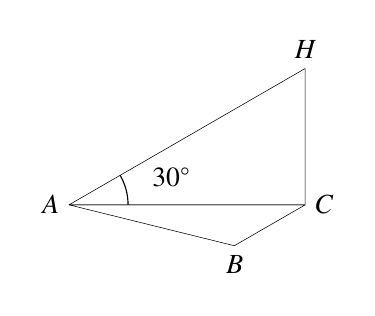
\begin{tikzpicture}[
  scale=1.5,
  decoration={
    markings,
    mark=at position 3cm with {\arrow[scale=2]{>}};
  }]
  % 初始化
  \tkzInit[xmin=-0.35,xmax=2.35, ymin=-0.7,ymax=1.5] \tkzClip    
  % 定义A、C坐标
  \tkzDefPoints{0/0/A, 2/0/C}  
  % 标记线段A、C点符号
  \tkzLabelPoints[left](A)
  \tkzLabelPoints[right](C)
  % 利用相对位置,用极坐标定义a点
  \tkzDefShiftPoint[A](30:1){a}
  % 利用相对位置,用极坐标定义h点
  \tkzDefShiftPoint[C](90:1){h}
  % 求Aa与Ch的交点H
  \tkzInterLL(A,a)(C,h) \tkzGetPoint{H}
  % 标记线段H点符号
  \tkzLabelPoints[above](H)

  % 定义过C点平行于HA,长度为0.3倍HA的的点B
  \tkzDefPointWith[colinear=at C,K=0.3](H,A) \tkzGetPoint{B}
  % 标记线段B点符号
  \tkzLabelPoints[below](B)

  % 用线段绘制三角形
  % \tkzDrawSegments(A,C)
  % \tkzDrawSegments(A,H)
  % \tkzDrawSegments(C,H)

  % \tkzDrawSegments(A,B)
  % \tkzDrawSegments(B,C)

  % 直接用多边形命令绘制三角形
  \tkzDrawPolygon(A, C, H)
  \tkzDrawPolygon(A, C, B)

  % 标记角度
  \tkzMarkAngle[size=0.5](C,A,H)
  \tkzLabelAngle[pos=0.9](C,A,H){$30^\circ$}
 \end{tikzpicture}
  
\end{document}

%%% Local Variables:
%%% mode: latex
%%% TeX-master: t
%%% End:
